\section{MIMA}

\begin{frame}{MIMA}
	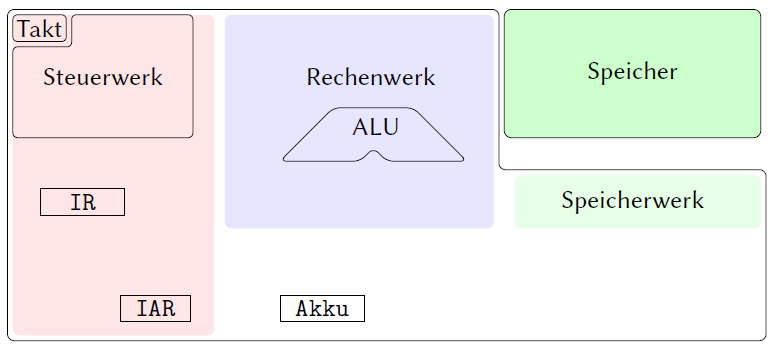
\includegraphics[width=\linewidth]{MIMA_simple.png}\\
	Die \emph{MIMA} ist ein idealisierter Prozessor. 
\end{frame}

\begin{frame}{Eigenschaften}
	\begin{itemize}[<+->]
		\item Adressen sind 20 Bit lang
		\item \enquote{Werte} sind 24 Bit lang
		\item Befehlscodierungen:
		\begin{itemize}
			\item 4 Bit für den OpCode und 20 Bit für einen Parameter (Adresse / Konstante)
			\item 8 Bit Befehl (Rest irrelevant)\\
			\includegraphics[width=100px]{MIMA_commands.png}\\
		\end{itemize} 
	\end{itemize}
\end{frame}


\begin{frame}{Wichtige Register}
	\begin{itemize}[<+->]
		\item \emph{IAR} : InstruktionsAdressRegister : Speichert Adresse des aktuell auszuführenden Befehls.
		\item \emph{IR}: InstruktionsRegister : Speichert den auszuführenden Befehl.
		\item \emph{SAR}: SpeicherAdressRegister : Enthält die Adresse eines Wertes, der aus dem Speicher gelesen werden soll.
		\item \emph{SDR}: SpeicherDatenRegister : Enthält einen Wert, der aus dem Speicher geladen wurde.
	\end{itemize}
\end{frame}

\begin{frame}{Aufbau}
	\begin{figure}
		\centering
		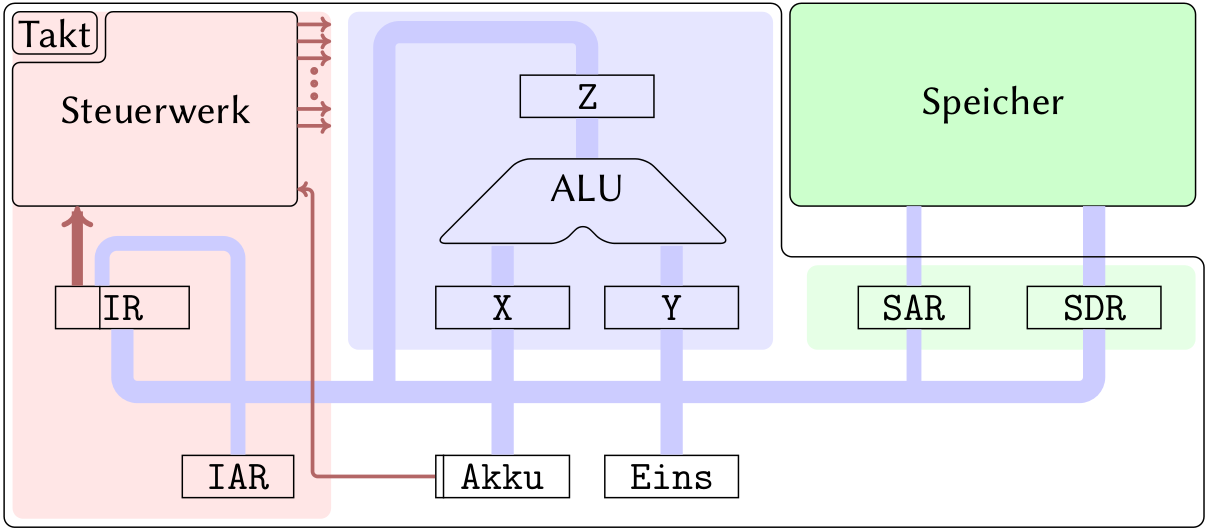
\includegraphics[width=\linewidth]{MIMA.png}
	\end{figure}
\end{frame}

\begin{frame}{Befehlsholphase}
	\begin{figure}
		\centering
		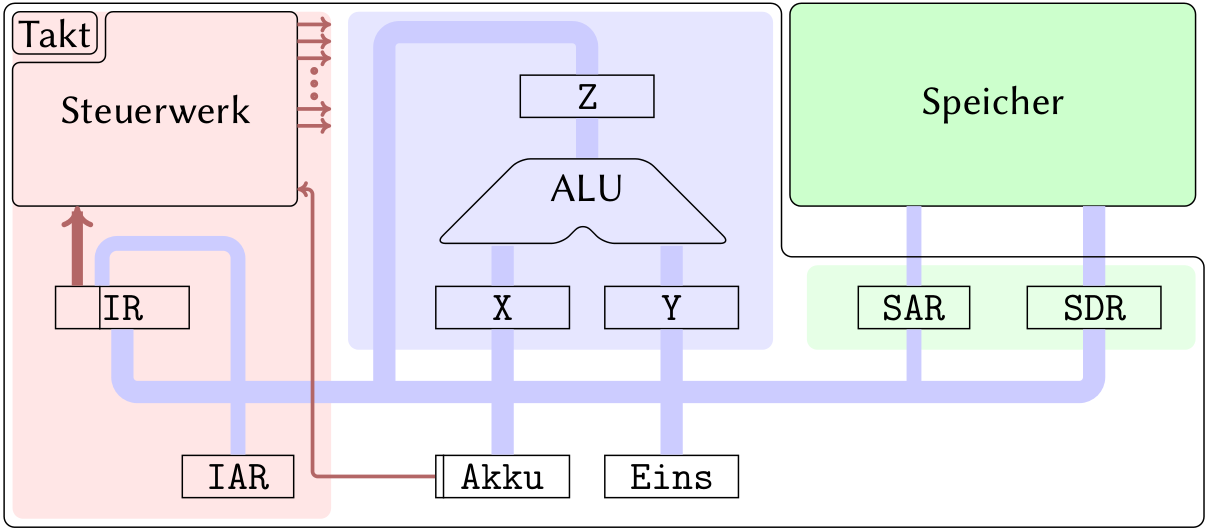
\includegraphics[width=\linewidth]{MIMA.png}
	\end{figure}
	\pause
	\only<2-6>{\begin{itemize}
		\only<2|handout:1> {\item[1] IAR $\to $ SAR  und IAR $\to$ X 
			\item[] Befehlsadresse dem Speicher übergeben und Zähler zum Erhöhen an ALU geben.}
		\only<3|handout:2>{\item[2] Eins $\to$ Y  
			\item[] 1-Wert für Erhöhung des Zählers an ALU geben.}
		\only<4|handout:3>{\item[3] ALU aufaddieren (Z=X+Y) 
			\item[] Nächste Befehlsadresse berechnen. }
		\only<5|handout:4>{\item[4] Z $\to$ IAR 
			\item[] Adresse für nächste Runde speichern. }
		\only<6|handout:5>{\item[5] SDR $\to$ IR 
			\item[] Wert zur angefragten Adresse erhalten. }
	\end{itemize}}	
\end{frame}

\begin{frame}{Befehle}
	Die MIMA besitzt einen Befehlssatz mit möglichen Befehlen. Andere Befehle (oder Varianten) werden NICHT unterstützt und können daher nicht verwendet werden!
	
	\begin{itemize}[<+->]
		\item Rechenoperationen
		\begin{itemize}
			\item ADD adr
			\item AND, OR, XOR adr
			\item NOT, RAR (keine Paramter)
		\end{itemize}
		\item Zugriffsoperationen
		\begin{itemize}
			\item LDC const (const ist dabei eine \textbf{20-Bit} Konstante)
			\item LDV, STV adr
			\item LDIV, STIV adr
		\end{itemize}
		\item Vergleichsoperation: EQL adr (-1 wenn gleich, 0 sonst)
		\item Sprünge
		\begin{itemize}
			\item JMP adr
			\item JMN adr (Jump if negative)
		\end{itemize}
		\item HALT
	\end{itemize}
\end{frame}

\begin{frame}{Bemerkungen}
	\begin{block}{Indirekte Adressierung}
		\centering
		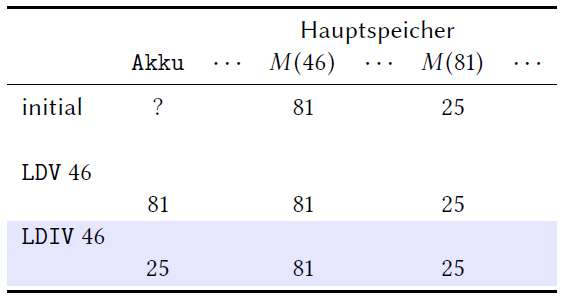
\includegraphics[width=150px]{MIMA_indirect.png}
	\end{block}
	
	\pause
	\begin{block}{HALT}
		Jedes Programm muss mit HALT enden! Sonst läuft das Programm endlos weiter!
	\end{block}

	\pause
	\begin{block}{Negative Konstanten}
		Negative Konstanten können nicht mit LDC geladen werden.\\
		Warum? \pause Unser Akku ist 24 Bit breit, aber wir können nur in die hinteren 20 Bit laden!
	\end{block}
\end{frame}

\begin{frame}{Negative Zahlen}
	\begin{block}{Aufgabe}
		Schreibe ein Programm, das von einer an Adresse $a_1$ gegebenen positiven Zahl das Zweierkomplement berechnet und an Adresse $a_2$ ablegt.
	\end{block}

	\visible<2|handout:2>{
		\begin{block}{Lösung}
			LDV $a_1$\\
			NOT\\
			STV $a_2$\\
			LDC 1\\
			ADD $a_2$\\
			STV $a_2$
		\end{block}
	}
\end{frame}

\begin{frame}{Beispiele}
	Beispiele zur Umsetzung von Answeisungen aus Hochsprachen:\\
	Siehe Übung
\end{frame}

\begin{frame}{Übung: Modulo}
	Schreibe ein Programm, das eine an Speicheradresse $a_1$ gegebenen Zahl Modulo R rechnet und an Adresse $a_2$ ablegt.
	\begin{itemize}
		\item Modulo 2
		\item Modulo 3
	\end{itemize}
\end{frame}

\begin{frame}{Lösung: Modulo 2}
	start:   LDC 1 //000000000000000000000001 \\
	$\qquad$ AND $a_1$ \\
	$\qquad$ STV $a_1$ \\
	$\qquad$ HALT
\end{frame}

\begin{frame}{Lösung: Modulo 3}
	start:   LDC 1 \\
	$\qquad$ STV One\\
	$\qquad$ LDC 3\\
	$\qquad$ NOT\\
	$\qquad$ ADD One\\
	$\qquad$ STV MThree\\
	\medskip
	while:   LDV MThree\\
	$\qquad$ ADD $a_1$\\
	$\qquad$ JMN abschluss\\
	$\qquad$ STV $a_1$\\
	$\qquad$ JMP while\\
	\medskip
	ende:    LDC 3\\
	$\qquad$ ADD $a_1$\\
	$\qquad$ HALT\\
\end{frame}